% It is an example file showing how to use the 'sigkddExp.cls' 
% LaTeX2e document class file for submissions to sigkdd explorations.
% It is an example which *does* use the .bib file (from which the .bbl file
% is produced).
% REMEMBER HOWEVER: After having produced the .bbl file,
% and prior to final submission,
% you need to 'insert'  your .bbl file into your source .tex file so as to provide
% ONE 'self-contained' source file.
%
% Questions regarding SIGS should be sent to
% Adrienne Griscti ---> griscti@acm.org
%
% Questions/suggestions regarding the guidelines, .tex and .cls files, etc. to
% Gerald Murray ---> murray@acm.org
%
 
\documentclass{sigkddExp}

\usepackage{booktabs} 
\usepackage{multirow, array}
\usepackage{makecell}
\usepackage[table,x11names]{xcolor}
\usepackage{enumitem}

\begin{document}

%
% --- Author Metadata here ---
% -- Can be completely blank or contain 'commented' information like this...
%\conferenceinfo{WOODSTOCK}{'97 El Paso, Texas USA} % If you happen to know the conference location etc.
%\CopyrightYear{2001} % Allows a non-default  copyright year  to be 'entered' - IF NEED BE.
%\crdata{0-12345-67-8/90/01}  % Allows non-default copyright data to be 'entered' - IF NEED BE.
% --- End of author Metadata ---

\title{6.864, Fall 2017 - Neural Approaches to Question Retrieval}
\subtitle{Codebase: https://github.com/shashank-srikant/6.864\_term\_project}

% You need the command \numberofauthors to handle the "boxing"
% and alignment of the authors under the title, and to add
% a section for authors number 4 through n.
%
% Up to the first three authors are aligned under the title;
% use the \alignauthor commands below to handle those names
% and affiliations. Add names, affiliations, addresses for
% additional authors as the argument to \additionalauthors;
% these will be set for you without further effort on your
% part as the last section in the body of your article BEFORE
% References or any Appendices.

\numberofauthors{2}
%
% You can go ahead and credit authors number 4+ here;
% their names will appear in a section called
% "Additional Authors" just before the Appendices
% (if there are any) or Bibliography (if there
% aren't)

% Put no more than the first THREE authors in the \author command
%%You are free to format the authors in alternate ways if you have more 
%%than three authors.

\author{
%
% The command \alignauthor (no curly braces needed) should
% precede each author name, affiliation/snail-mail address and
% e-mail address. Additionally, tag each line of
% affiliation/address with \affaddr, and tag the
%% e-mail address with \email.
\alignauthor Vadim Smolyakov*\\
       \affaddr{CSAIL, MIT}\\
       \email{vss@csail.mit.edu}
\alignauthor Shashank Srikant\titlenote{Author order decided by tossing a fair coin.}\\
       \affaddr{CSAIL, MIT}\\
       \email{shash@mit.edu}
}

\balancecolumns
\date{30 July 1999}
\maketitle
\begin{abstract}
Content on the internet grows at an exponential rate. Given this growth, finding relevant information accurately becomes a critical task for the NLP community to address. More so, with this rapid growth, curating labeled datasets to build models for the wide variety of content available on the internet has become extremely time and resource intensive. In this work, we explore whether neural models are able to successfully model content similarity and retrieval tasks, and whether they can transfer knowledge from one domain, where supervised labels are available, to a domain with no available labels. Specifically, we explore content similarity in online discussion forums, where we explore the following questions - a. how effectively can neural approaches model question-answer retrieval tasks, which is, given a question and answer pair present on an online discussion forum, how effectively can neural approaches find similar pairs on that forum. b. Given a model of question-answer similarity in one online discussion forum, how effective are neural approaches in transferring that knowledge to a new, loosely related domain. In this work, we explore a baseline approach of modeling question similarity tasks on the popular online community  \textit{AskUbuntu}. We show how neural architectures like LSTMs and CNNs outperform traditional approaches in information retrieval. Additionally, and importantly, we explore the problem of transferring these models to detect question-answer similarity on \textit{Android stack exchange},  a similar yet different online discussion community which discusses Android related problems. We show how neural domain adaptation techniques successfully beat baseline IR techniques and direct neural transfer techniques. We also discuss some limitations and challenges in using such architectures.
\end{abstract}

\begin{table*}[th]
\begin{tabular*}{\linewidth}{m{0.13\linewidth}m{0.12\linewidth}m{0.18\linewidth}m{0.18\linewidth}m{0.28\linewidth}}
\toprule
\toprule
\textbf{Scenario} & \textbf{Setting} & \textbf{Nature of Data} & \textbf{Learning Paradigm} & \textbf{Main Concepts}  \\
\toprule 
 \makecell{$\mathcal{D}_S = \mathcal{D}_T,$\\$ T_S = T_T$}
& Traditional Machine learning
& Labelled data in source domain(s) and unlabeled data in target domain
& Source and target domains are exactly the same
& Learn models on training set and test on future unseen data \\
\cmidrule{1-5}
 \multirow{2}{\linewidth}{\textbf{\makecell{$\mathcal{D}_S \neq \mathcal{D}_T$,\\ $T_S = T_T$}}} 
& \multirow{2}{\linewidth}{Transductive Transfer Learning}
& \multirow{2}{\linewidth}{Labelled data in source domain(s) and unlabeled data from $\mathcal{P}(X_S) \neq \mathcal{P}(X_T$)}
& Single source domain adaptation
\cellcolor{blue!25}
& Learning common shared representation; instance weighing, parameter transfer
\\
\cmidrule{4-5}
 
&
&
& Multi-source adaptation
& Classifier combination; efficient combination of information from multiple sources; Feature representation \\
\cmidrule{1-5} 

\multirow{2}{\linewidth}{No conditions on $\mathcal{D}_S$, $\mathcal{D}_T$, 
but $T_S \neq T_T$ }
& \multirow{2}{\linewidth}{Inductive Transfer Learning}
& Unlabeled data in source domain(s) and labeled data in target domain
& Self-taught learning
& Extracts higher level representations from unlabeled auxiliary data to learn instance-to-label mapping with labeled target instances
\\
\cmidrule{3-5} 
& & Labeled data is available in all domains
& Multi-task learning
& Simultaneously learns multiple tasks within (or across) domain(s) by exploiting the common feature subspace shared across the tasks \\
\cmidrule{1-5}
\makecell{$\mathcal{D}_S\neq \mathcal{D}_T$\\$T_S \neq T_T$}
& Kim et al., 2015 \cite{kim2015new}
& Labeled data in source and target domains
& Transfer learning with disparate label set
& Disparate fine grained label sets across domains, however, same coarse grained labels set can be invoked across domains
\\
\bottomrule
\end{tabular*}
\caption {A brief summary of different transfer learning approaches. The cell marked in blue highlights the approach explored in this work. This summary is based on the work detailed in the survey paper by Pan et. al.\protect\cite{pan2010survey}}
\label{tab:related_work}
\end{table*}

\section{Introduction}
The problem of text similarity, and specifically, similarity of short queries or answers found on the internet, have been central to the modern NLP community. With the explosion in content on the internet, a lack of robust tools to find similar content has the risk of creating further similar and redundant content, which only exacerbates the original problem.

Another relevant and pressing concern which such an explosion and variety of content has introduced is the increased cost of building predictive NLP, NLU models which cater to such content. The variety in content requires building a model from scratch, irrespective of how closely related the content may have been to a previously built model. For instance, if we were to model the reviews written for movies, we would have to reinvest effort and time in modeling reviews written for another domain, say, food or hotels. In spite there being conceptual, semantic similarities between the tasks of reviewing movies and reviewing food, models have to be created anew. And each such modeling exercise demands a large repository of curated, preferably labeled data, which most often is not feasible to put together. The pressing challenge such a variety of content has created is to be able to learn with minimal supervision, and from loosely related datasets.

In this work, we investigate two problems - one, to model question-similarity tasks using state of the art techniques in neural modeling and two, transfer those models to a loosely related, yet equally rich domain under the constraint of having no supervised information on that new domain. Specifically, we explore the problem of finding similar question-answer pairs on the popular online discussion \textit{AskUbuntu}.\footnote{https://askubuntu.com} This discussion forum focuses on troubleshooting queries on Ubuntu, the popular open-source operating system. In addition to  learning models to find relevant question-answer pairs on this forum, we also use this domain to transfer knowledge onto modeling question-answer similarity in \textit{Android stack exchange}.\footnote{https://android.stackexchange.com} This is an online community, similar in setup and structure to \textit{AskUbuntu}, wherein short queries and corresponding answers on Android-related troubleshooting are present.

In this work, we investigate how state of the art neural architectures for NLP applications perform on the task of question similarity. Traditionally, text similarity tasks were solved using information retrieval techniques like building an indexer and applying ABC and ABC, which consider XYZ. We study how more recent techniques like RNNs and CNNs, which have shown to successfully model text on tasks like XYZ, model this particular task. For the domain adaptation task of learning question similarity in {Android stack exchange}, we explore adversarial neural techniques, and Doc2Vec \cite{REF} in learning from the \textit{Ask Ubuntu} dataset. 

The study demonstrates the relevance of neural techniques in a critical NLP task like question-answer retrieval. We demonstrate how using neural approaches, one can outperform traditional information retrieval techniques while not having to invest heavily in engineering the right features to get to such a performance. Additionally, we show the successful transfer of domain knowledge from one domain to another using state of the art neural transfer techniques.

This work is organized into the following sections - Section \ref{related} discusses related work in this field. Sections \ref{in_domain}, \ref{domain_adapt},  \ref{other_techniques} discuss the various techniques to model in-domain and domain adaptation tasks for the given problem. Section \ref{experiments} discusses the experiment setup and the results. Section \ref{discussion} discusses the results and concludes our work.


\begin{figure*}[h]
\centering
\begin{tabular}{cc}
    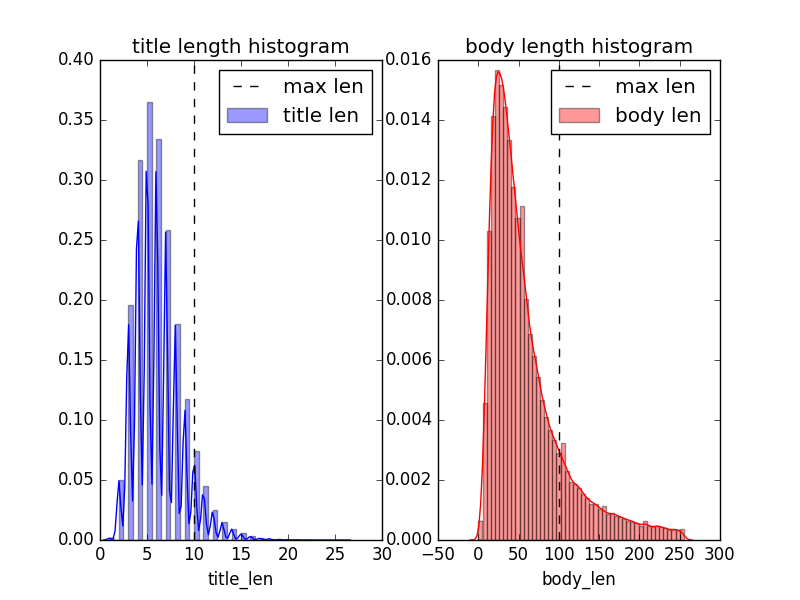
\includegraphics[width=\columnwidth]{img/question_len_hist}
&   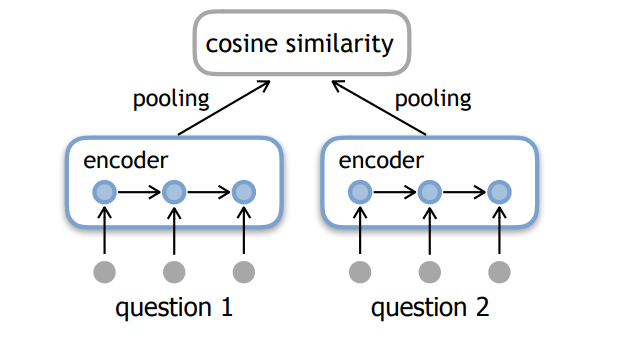
\includegraphics[width=\columnwidth]{img/similar}
\\
   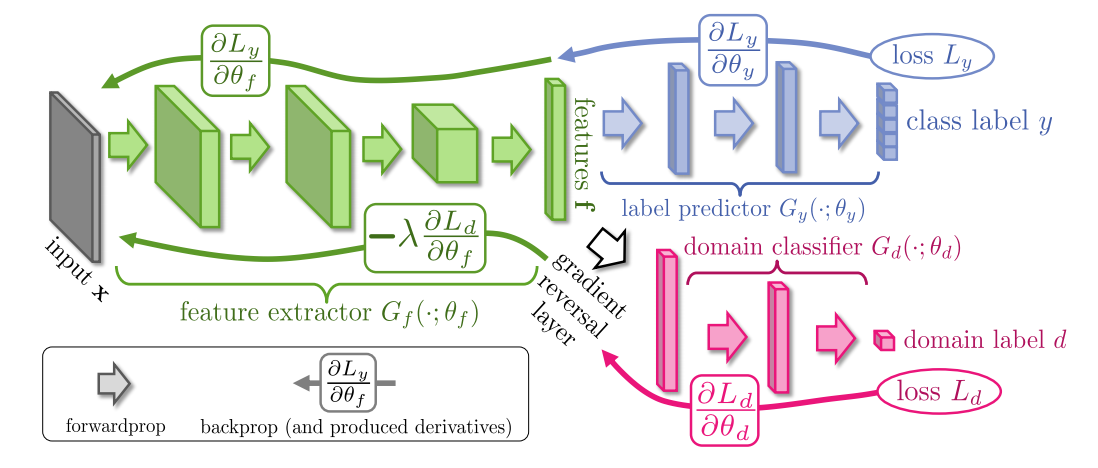
\includegraphics[width=\columnwidth]{img/adversary}
&   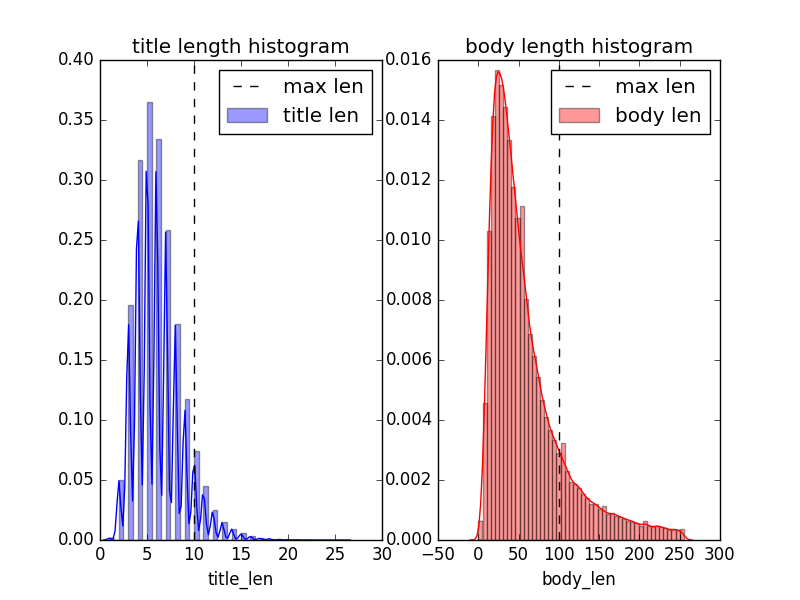
\includegraphics[width=\columnwidth]{img/question_len_hist}
\end{tabular}
\label{fig:len_hist}
\caption{Summary of the \textit{Ask Ubuntu} dataset}
\end{figure*}

\section{Related work}
\label{related}
Given the growing popularity of community QA forums, question retrieval has emerged as an important area of research. Recent work has also gone beyond word-based methods to represent this task. For instance, Feng et. al. \cite{feng2015applying} learn word embeddings using category-based metadata information for questions. They define each question as a distribution which generates each word (embedding) independently, and subsequently use a Fisher kernel to assess question similarities. Dos Santos et. al. \cite{dos2015learning} propose an approach which combines a convolutional neural network (CNN) and a bag of words representation for comparing questions. In contrast to \cite{feng2015applying}, Lei et. al. \cite{lei2015semi} treat each question as a word sequence as opposed to a bag of words, and apply recurrent CNNs instead of traditional CNNs. We base our work on \cite{lei2015semi}. We apply different off-the-shelf deep learning models to encode a meaningful embedding and define similarity over these embeddings.

Domain adaptation has been an active area of research in NLP. Table \ref{tab:related_work}  summarizes different settings of transfer learning \cite{pan2010survey}. Our work explores techniques in unsupervised domain adaptation, which operates when the source and target domains ($\mathcal{D}$) are different, but share a common task ($T_i$) to achieve. It helps understand where this approach lies in the spectrum of techniques. 

We study in this work the scenario where the domains vary while the tasks remain the same. This is referred to as transductive transfer learning. This is the most extensively studied settings in the transfer learning literature and can be broadly categorized as single and multi-source adaptation. Single source adaptation\cite{chen2009extracting, ando2005framework, daume2009frustratingly} primarily aims at minimizing the divergence between the source and target domains either at instance or feature levels. The general idea being identifying a suitable low dimensional space where transformed source and target domains data follow similar distributions and hence, a standard supervised learning algorithm can be trained.

Multiple methods perform unsupervised domain adaptation by matching the feature distributions in the source and the target domains. Some approaches perform this by reweighing or selecting samples from the source domain  \cite{borgwardt2006integrating, huang2007correcting, gong2012geodesic}, while others seek an explicit feature space transformation that would map source distribution into the target ones \cite{pan2011domain, gopalan2011domain, baktashmotlagh2013unsupervised}. An important  aspect of the distribution matching approach is the way the (dis)similarity between distributions is measured. Here, one popular choice is matching the distribution means in the kernel-reproducing Hilbert space \cite{borgwardt2006integrating, huang2007correcting}, whereas \cite{gong2012geodesic, fernando2013unsupervised} map the principal axes associated with each of the distributions. The approach explored in this work is based on \cite{ganin2015unsupervised} and also attempts to match feature space distributions, however this is accomplished by modifying the feature representation itself rather than by reweighing or geometric transformation. Also, the method used to measure the disparity between distributions based on their separability is implicitly different and is done by a deep discriminatively-trained classifier.


\section{In-domain Question similarity}
\label{in_domain}
We first explore the task of question similarity by training a domain-specific classifier. The domain we have explored in this work involves the questions and answers asked on \textit{AskUbuntu}, a popular online discussion forum where the community troubleshoots problems related to Ubuntu, the operating system. The dataset for this task was curated by \cite{lei2015semi}. 

\begin{table}[h]
\begin{tabular}{l|r|r}
     
     & $\mathsf{source} (\mathcal{D_S})$
     & $\mathsf{target} (\mathcal{D_T})$
     \\
     \toprule
     Description
     & \textit{Ask Ubuntu}
     & \textit{Android SE}
     \\
     \# of sentences
     & 40
     & 50
     \\
     \# of stop words 
     & 50
     & 90
     \\
     mean word length - title
     & 299
     & 300
     \\
     mean word length - body
     & 299
     & 300
\end{tabular}
\caption{Summary statistics of our dataset}
\label{tab:dataset}
\end{table}

\subsection{Dataset}
We describe here the dataset that we base our work on.
\begin{itemize}[topsep=0pt,itemsep=-1ex,partopsep=1ex,parsep=1ex]
\item The \textit{Ask Ubuntu} dataset consists of question and answers related to problems people face in Ubuntu, the operating system
\item Each query has two components - a title and main body. The average title length is XX words and the average body length is YY words long. Figure \ref{fig:len_hist} shows the distribution of word lengths.
\item In this work, to limit computational requirement, we consider only the first XX words in the title and the first YY words in the body of each sentence.
\item The \textit{Ask Ubuntu} platform has a section where users flag similar questions. We use that as a weak signal to inform our true labels, since these user-flagged suggestions are not complete and suffer from high recall issues.
\item In order to train our classifiers with dissimilar pairs of questions, each query is also associated with randomly drawn queries from the sample.
\item We trained on roughly 110,000 query-answer pairs to train our in-domain classifier.
\item In the test set, for each pair of similar and dissimilar questions, we are also given the $\mathsf{BM25 scores}$, their similarity as measured by an industrial IR-system. These serve as a baseline for all our experiments.
\end{itemize}

\subsection{Model}
We model the task of in-domain question similarity as follows:
\begin{itemize}[topsep=0pt,itemsep=-1ex,partopsep=1ex,parsep=1ex]
  \item We define a word-level deep neural network. The network takes in a word at a time, and is represented by embeddings.  This word can either belong to the title or the body of a query. In this work, we average the embeddings from the title and body of each query, and use the averaged embeddings to classify similarity.
  \item We use pre-trained embeddings on data drawn from both, the source domain and Wikipedia. Both these data sources are rich, are easily available and training these embeddings using Word2Vec etc. are relatively straightforward.
  \item To train the classifier to find similar and dissimilar questions for a given query, we associate each query with two sets of texts - the set of similar questions as marked by users on \textit{Ask Ubuntu}, and 100 randomly sampled questions from the corpus which serve as dissimilar pairs. The user-defined questions are used only during training. Since user-marked similar questions are not comprehensive and serve only as a weak proxy, the system is tested on expert-marked similar questions.
  \item In this setup, we find the distances between a query and its similar questions and dissimilar questions by defining a similarity operation over its embeddings. We use the cosine distance between the embeddings as a similiarity operation.
  \item We use a maxmargin framework for learning parameters $\theta$ of our network. Specifically, in a context of a particular training example where $q_i$ is paired with $p^+_i$, we minimize the max-margin loss $L(\theta)$ defined as\\
  \begin{equation}
  \max_{p^- \in Q(q_i)} \{s(q_i,p^-;\theta) - s(q_i,p^+_i;\theta) + \delta(p, p^+_i)\}
  \end{equation}
where $\delta(.,.)$ denotes a non-negative margin. We set $\delta(p, p^+_i)$ to be a small constant when $p \neq p^+_i$ and 0 otherwise. The parameters $\theta$ can be optimized through sub-gradients ${\partial L}/{\partial \theta}$ aggregated over small batches of the training instances \cite{lei2015semi}.
  \item The neural network essentially serves as an encoder to generate a representation in a low-dimension space which encodes the loss function $L(.)$ defined above.
  \item In this work, we implement two neural networks, LSTMs and CNNs, as these encoders.
\end{itemize}

\begin{table}[h]
\begin{tabular}{l|r|l|r}
      \multicolumn{2}{c|}{CNN}
     & \multicolumn{2}{c}{LSTM}
     \\
     \toprule
     Parameter
     & Value
     & Parameter
     & Value
     \\
     \# of sentences
     & 40
     & \# of sentences
     & 50
     \\
     \# of stop words 
     & 50
     & \# of sentences
     & 90
     \\
     mean word length - title
     & 299
     & \# of sentences
     & 300
     \\
     mean word length - body
     & 299
     & \# of sentences
     & 300
\end{tabular}
\caption{Parameters of our encoder networks for in-domain classification}
\label{tab:indomain}
\end{table}

\subsection{CNN}
We describe the CNN architecture implemented in this work. We detail the inputs to the different layers of the network, which should help illustrate the architecture.
We define a CNN with the following layers -
\begin{itemize}[topsep=0pt,itemsep=-1ex,partopsep=1ex,parsep=1ex]
\item \textbf{Input vector $\mathbf{X}$} of dimensions: ($\mathbf{B}$, $\mathbf{W}$) ($\mathbf{B}$: batch size, $\mathbf{W}$: max \# of words in sentence in batch)
\item \textbf{Embedding layer} Pass $\mathbf{X}$ through embeddings layer. Resulting dimension: ($\mathbf{B}$, $\mathbf{W}$, $\mathbf{D}$) ($\mathbf{D}$: \# of embeddings per word)
\item \textbf{Convolution, ReLU} Pass the above input through a convolution layer and then through ReLU. Resulting dimension: ($\mathbf{B}$, $\mathbf{K}$, $\mathbf{Y}$)($\mathbf{K}$: Depth of filter, i.e. \# of filters of given height, $\mathbf{Y}$: \# of values sliding the filter over the input)
\item \textbf{Pooling} Pass through mean pooling. Resulting dimension: ($\mathbf{B}$, $\mathbf{K}$)
\item The resulting encoded embedding of dimension ($\mathbf{B}$, $\mathbf{K}$) for $\mathbf{B}$ words in a given batch.
\end{itemize}

\subsection{LSTM}
We describe the CNN architecture implemented in this work. We detail the inputs to the different layers of the network, which should help illustrate the architecture.
We define a CNN with the following layers -
\begin{itemize}[topsep=0pt,itemsep=-1ex,partopsep=1ex,parsep=1ex]
\item \textbf{Input vector $\mathbf{X}$} Dimensions: ($\mathbf{B}$, $\mathbf{W}$) ($\mathbf{B}$: batch size, $\mathbf{W}$: max \# of words in sentence in batch)
\item \textbf{Embedding layer} Pass $\mathbf{X}$ through embeddings layer. Resulting dimension: ($\mathbf{B}$, $\mathbf{W}$, $\mathbf{D}$) ($\mathbf{D}$: \# of embeddings per word)
\item \textbf{Convolution, ReLU} Pass the above input through a convolution layer and then through ReLU. Resulting dimension: ($\mathbf{B}$, $\mathbf{K}$, $\mathbf{Y}$)($\mathbf{K}$: Depth of filter, i.e. \# of filters of given height, $\mathbf{Y}$: \# of values sliding the filter over the input)
\item \textbf{Pooling} Pass through mean pooling. Resulting dimension: ($\mathbf{B}$, $\mathbf{K}$)
\item The resulting encoded embedding of dimension ($\mathbf{B}$, $\mathbf{K}$) for $\mathbf{B}$ words in a given batch.
\end{itemize}

\section{Domain Adaptation (DA)}
\label{domain_adapt}
We use neural adversarial techniques\cite{ganin2015unsupervised} to adapt to a domain having no labeled data, having trained a model on a domain with labeled data. In this section and the next, we describe the dataset we worked on, the architecture for the adversarial model we use, and other models for DA we tried.


\subsection{Dataset}
We worked with two datasets, one as our $\mathsf{source}$ domain, wherein we had labeled data and another as our $\mathsf{target}$ domain, where we had no labeled data. The task on both these datasets was the same - to predict similarity between questions. The $\mathsf{source}$ domain in our experiments was the \textit{Ask Ubuntu} dataset, described in the previous section. The $\mathsf{target}$ domain that we wanted to transfer this model to was the \textit{Android stack exchange}, a question-answer site on Android-related issues. Table \ref{tab:dataset} describes the summary statistics of this dataset. For the $\mathsf{target}$ domain, we had XX sentences to test. Each query was expert-annotated with similar and dissimilar queries they corresponded to. No $\mathsf{BM25 scores}$ were provided to evaluate a baseline. Table XX describes the architecture of the encoders and decoders.

\begin{table*}[h]
\parbox{.55\linewidth}{
    
    \begin{tabular}{l|r|l|r}
          \multicolumn{2}{c|}{CNN}
         & \multicolumn{2}{c}{LSTM}
         \\
         \toprule
         Parameter
         & Value
         & Parameter
         & Value
         \\
         \# of sentences
         & 40
         & \# of sentences
         & 50
         \\
         \# of stop words 
         & 50
         & \# of sentences
         & 90
         \\
         mean word length - title
         & 299
         & \# of sentences
         & 300
         \\
         mean word length - body
         & 299
         & \# of sentences
         & 300
    \end{tabular}
    \caption{Parameters of the encoder and domain differentiator\protect\\ networks for domain adaptation}
    \label{tab:indomain}
}
\parbox{.5\linewidth}{
    
    \begin{tabular}{l|r|l|r}
          \multicolumn{2}{c|}{Siamese}
         & \multicolumn{2}{c}{$\mathsf{doc2vec}$}
         \\
         \toprule
         Parameter
         & Value
         & Parameter
         & Value
         \\
         \# of sentences
         & 40
         & \# of sentences
         & 50
         \\
         \# of stop words 
         & 50
         & \# of sentences
         & 90
         \\
         mean word length - title
         & 299
         & \# of sentences
         & 300
         \\
         mean word length - body
         & 299
         & \# of sentences
         & 300
    \end{tabular}
    \caption{Parameters of $\mathsf{doc2vec}$ and the siamese network architectures}
    \label{tab:indomain}
}
\end{table*}

\subsection{Model}
We model this task of unsupervised domain adaptation using a neural adversarial approach \cite{ganin2015unsupervised}. The core idea is as follows - 
\begin{itemize}[topsep=0pt,itemsep=-1ex,partopsep=1ex,parsep=1ex]
    \item We define an encoder which is able to take in the data from the $\mathsf{source}$ domain and learn a representation which predicts the similarity for tasks in its own domain, given that we have labels for this domain. This is similar to the in-domain learning described in the previous section.
    \item While the primary goal of predicting $\mathcal{Y}_\mathsf{source}$ remains, we define an adversarial objective to guide the direction of the encoded embeddings in a way to make them abstract enough to be able to discriminate $\mathcal{Y}_\mathsf{target}$ as well.
    \item We do this by setting an objective in the adversarial to predict the label $\mathsf{source}$ or $\mathsf{target}$. If the origin of the input data is being discriminated well by the adversarial network, a negative weight is propagated to the encoder, thereby making the encoding abstract enough to not being able to distinguish between the two domains, while being able to predict $\mathcal{Y}_\mathsf{source}$ well. This ensures the successful transfer of the encoded embeddings to the $\mathsf{target}$ domain. Figure \ref{fig:adversary} depicts this arrangement.
\end{itemize}


\begin{figure}[h]
\centering
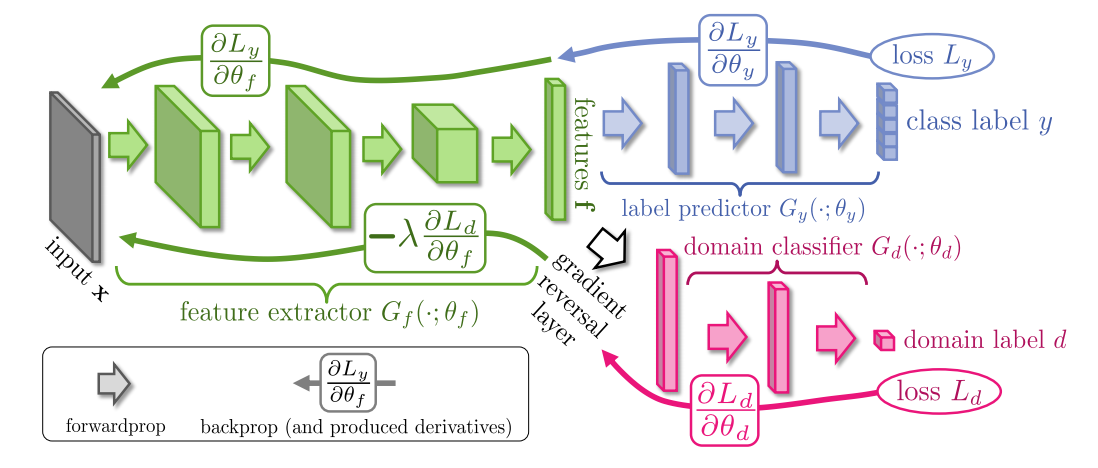
\includegraphics[width=\columnwidth]{img/adversary.png}
\label{fig:adversary}
\caption{Adversarial network for unsupervised domain adaptation investigated in this work. Image reference: Ganin et al., 2015 \protect\cite{ganin2015unsupervised}}
\end{figure}
    
\section{Other techniques for DA}
\label{other_techniques}
We explored two other techniques to carry out unsupervised domain transfer. We tried out Doc2Vec \cite{doc2vec1} and Siamese recurrent networks \cite{siamese} for domain transfer. We describe each briefly here:

\begin{itemize}[topsep=0pt,itemsep=-1ex,partopsep=1ex,parsep=1ex]
\item \textbf{Doc2Vec} Paragraph vectors, or $\mathsf{doc2vec}$, were proposed by Le and Mikolov (2014) as a simple extension to word2vec to extend the learning of embeddings from words to word sequences. $\mathsf{doc2vec}$ is agnostic to the  granularity of the word sequence — it can equally be a word n-gram, sentence, paragraph or document. In this paper, we use the term ``document embedding'' to refer to the embedding of a word sequence, irrespective of its granularity.

\item \textbf{Siamese networks} 

\end{itemize}

\section{Experiments}
\label{experiments}
We pose the following research questions, whose answers we investigate in this work
\begin{itemize}[topsep=0pt,itemsep=-1ex,partopsep=1ex,parsep=1ex]
\item \textbf{E1:} How well do deep neural encoders solve the task of in-domain question retrieval. How does it compare to baselines and the state of the art? What are the limitations.
\item \textbf{E2:} How effective are deep adversarial neural methods in adapting from one domain to another to learn a common task. How does it compare to the baselines and state of the art? What are the limitations?
\item \textbf{E3:} How effective is $\mathsf{doc2vec}$ in adapting knowledge from one domain to another.
\item \textbf{E4:} How effective are siamese networks in adapting knowledge from one domain to another.
\end{itemize}

\subsection{Experiment 1}
To answer $E1$, we measure the performance of our neural encoders against of $\mathsf{BM25 scores}$ provided for the test set of the corpus. The metrics we compare on 
\subsection{Experiment 2}
\subsection{Experiment 3}
\subsection{Experiment 4}

\section{Results}

\section{Discussion}
\label{discussion}

%ACKNOWLEDGEMENTS are optional
\section{Acknowledgements}
\label{ack}
The authors thank the course staff of 6.864, Fall 2017, MIT. This was a fun project!

%
% The following two commands are all you need in the
% initial runs of your .tex file to
% produce the bibliography for the citations in your paper.
\bibliographystyle{abbrv}
\bibliography{sigproc}  % sigproc.bib is the name of the Bibliography in this case
% You must have a proper ".bib" file
%  and remember to run:
% latex bibtex latex latex
% to resolve all references
%
% ACM needs 'a single self-contained file'!
%
%APPENDICES are optional
% SIGKDD: balancing columns messes up the footers: Sunita Sarawagi, Jan 2000.
% \balancecolumns

% That's all folks!
\end{document}
